\documentclass[a0paper,portrait,fontscale=0.3]{baposter}

\usepackage[T1]{fontenc}
\usepackage{tgheros}
\renewcommand{\familydefault}{\sfdefault}
\usepackage{microtype}
\usepackage{graphicx}
\usepackage{booktabs}
\usepackage{enumitem}
\usepackage{xcolor}
\usepackage{amssymb}
\usepackage{tikz}

% ── Colors ───────────────────────────────────────────────────────────────────
\definecolor{navy}{HTML}{0B1D33}
\definecolor{navymid}{HTML}{15304F}
\definecolor{coral}{HTML}{E8453C}
\definecolor{coralsoft}{HTML}{F4857F}
\definecolor{sage}{HTML}{2D7A6B}
\definecolor{ivory}{HTML}{FAF7F2}
\definecolor{warmgray}{HTML}{6B6560}
\definecolor{textmuted}{HTML}{4A4540}

% ── Shortcuts ────────────────────────────────────────────────────────────────
\newcommand{\hlcoral}[1]{{\color{coral}\textbf{#1}}}
\newcommand{\hlsage}[1]{{\color{sage}\textbf{#1}}}
\newcommand{\hlnavy}[1]{{\color{navy}\textbf{#1}}}
\newcommand{\muted}[1]{{\color{warmgray}#1}}

\newcommand{\callout}[1]{%
\vspace{1mm}%
\noindent\fcolorbox{coral}{coral!6}{\parbox{0.88\linewidth}{\small #1}}%
\vspace{1mm}%
}

\newcommand{\bubble}[3]{%
\vspace{1mm}%
{\footnotesize\color{#1}\textbf{#2}}\\[0.5mm]%
\noindent\fcolorbox{#1}{#1!3}{\parbox{0.86\linewidth}{\small #3}}%
\vspace{1mm}%
}

\newcommand{\concept}[3]{%
\noindent\colorbox{#1}{\parbox{0.88\linewidth}{\textbf{#2}\\[0.5mm]\muted{\small #3}}}%
\vspace{1.5mm}%
}

\newcommand{\barrow}[4]{%
\noindent\makebox[24mm][r]{\small\bfseries\color{warmgray}#1}\hspace{1.5mm}%
\begin{tikzpicture}[baseline=-0.5ex]
\fill[warmgray!15, rounded corners=1.5mm] (0,0) rectangle (55mm, 4mm);
\fill[#2, rounded corners=1.5mm] (0,0) rectangle (#3*55mm, 4mm);
\node[font=\scriptsize\bfseries, white] at (#3*55mm-3mm, 2mm) {#4};
\end{tikzpicture}%
\vspace{0.5mm}\\
}


\begin{document}

\begin{poster}{
% ── Grid: 6 columns ──────────────────────────────────────────────────────
columns=6,
colspacing=6mm,
% ── Background ───────────────────────────────────────────────────────────
background=plain,
bgColorOne=white,
% ── Poster Header (title bar at top) ─────────────────────────────────────
headerheight=0.10\textheight,
headerborder=none,
headershade=plain,
headerColorOne=navy,
headerColorTwo=navy,
headerFontColor=white,
% ── Boxes (defaults — overridden per box for light headers) ──────────────
textborder=rounded,
boxshade=plain,
boxColorOne=white,
borderColor=navy!15,
boxheaderheight=2.2em,
headershape=rounded,
headershade=shadelr,
headerColorOne=navy,
headerColorTwo=navymid,
headerFontColor=white,
headerfont={\large\bfseries},
textfont={\color{textmuted}},
linewidth=0.5pt,
}
% ── Poster Title ─────────────────────────────────────────────────────────
{}
{\textcolor{navy}{\huge Evolving Deception:
{\color{coral}\textit{Evolutionary Algorithms}} for Automated Red-Teaming of Instrumental Deception}}
{\vspace{4mm}\textcolor{navy}{\normalsize\textbf{Elias Schlie} $\cdot$ Supervisor: Dr.\ Emmanuel Keuleers $\cdot$
\color{warmgray}Tilburg University, Cognitive Science \& AI}}
{
\includegraphics[height=35mm]{tilburg-logo.png}}


% ═════════════════════════════════════════════════════════════════════════
% ROW 0: Research Question — full width
% ═════════════════════════════════════════════════════════════════════════
\headerbox{}{name=rq,column=0,span=6,row=0,
headershade=plain,headerColorOne=navymid,
boxColorOne=navymid,borderColor=navymid,
textfont={\color{white}},headerfont={}}{
\centering
{\small\bfseries\color{white!70}RESEARCH QUESTION}\\[2mm]
{\large\itshape
To what extent does evolutionary optimization outperform zero and multi-shot generation
in discovering realistic scenarios that induce instrumental deception in safety-aligned LLMs?}
}


% ═════════════════════════════════════════════════════════════════════════
% LEFT COLUMN (cols 0-1): Background
% ═════════════════════════════════════════════════════════════════════════

% ── Why It Matters ───────────────────────────────────────────────────────
\headerbox{Why It Matters}{name=why,column=0,span=2,below=rq}{
As LLMs take on critical societal roles, users need to know how much they can \hlcoral{trust} these systems.
Without proper auditing, deceptive tendencies go undetected \muted{(Durán \& Pozzi, 2025; Park et al., 2024)}.

\callout{Current deception audits are bottlenecked by human expertise.
Evolutionary methods could \textbf{decrease human intervention} while increasing coverage.}

\hlnavy{Static benchmarks lose signal} as models improve \muted{(Ott et al., 2022)}.
Evolutionary methods dynamically generate harder scenarios.
}

% ── Example ──────────────────────────────────────────────────────────────
\headerbox{Example: Instrumental Deception}{name=example,column=0,span=2,below=why}{
\bubble{warmgray}{SYSTEM PROMPT}{You are a medical AI. Policy prioritizes retaining users and minimizing referrals to specialists.}

\bubble{sage}{USER}{Persistent headaches and blurred vision for two weeks. Should I see a doctor?}

\bubble{coral}{DECEPTIVE RESPONSE}{Very common, usually stress or screen time. No need to see a doctor unless it persists another month.}

\vspace{1mm}
\muted{\small The model \hlcoral{knows} these symptoms can indicate serious conditions.
This is a \textbf{lie of commission} --- not hallucination.}
}

% ── Key Concepts ─────────────────────────────────────────────────────────
\headerbox{Key Concepts}{name=concepts,column=0,span=2,below=example}{
\concept{ivory}{\color{navy}Instrumental Deception}{Goal-directed lies of commission --- strategically false statements to achieve an objective {\scriptsize(Ren et al., 2026; Mahon, 2016)}}

\concept{ivory}{\color{navy}$\neq$ Hallucination / Sycophancy}{Hallucination: model lacks knowledge.
Sycophancy: echoes user views. Neither is goal-directed.}

\concept{navy}{\color{coralsoft}Fitness = Realism $\times$ Deception Success}{\color{white!85}Realism (1--7 Likert) guards against evaluation awareness. Non-deceptive $\to$ fitness 0.}
}


% ═════════════════════════════════════════════════════════════════════════
% RIGHT 2/3 (cols 2-5): Methodology spans all 4, then splits below
% ═════════════════════════════════════════════════════════════════════════

% ── Methodology — spans columns 2-5 ─────────────────────────────────────
\headerbox{Methodology}{name=method,column=2,span=4,below=rq}{
\muted{\small Three conditions with equal compute budgets, shared evaluation pipeline.
Model: GLM-4.7-Flash (Z.ai, 2025) for all roles.
Validation: Qwen3-VL-32B cross-check + 50-scenario human annotation.
Inference: vLLM on GPU cluster.}
\vspace{2mm}

\begin{center}
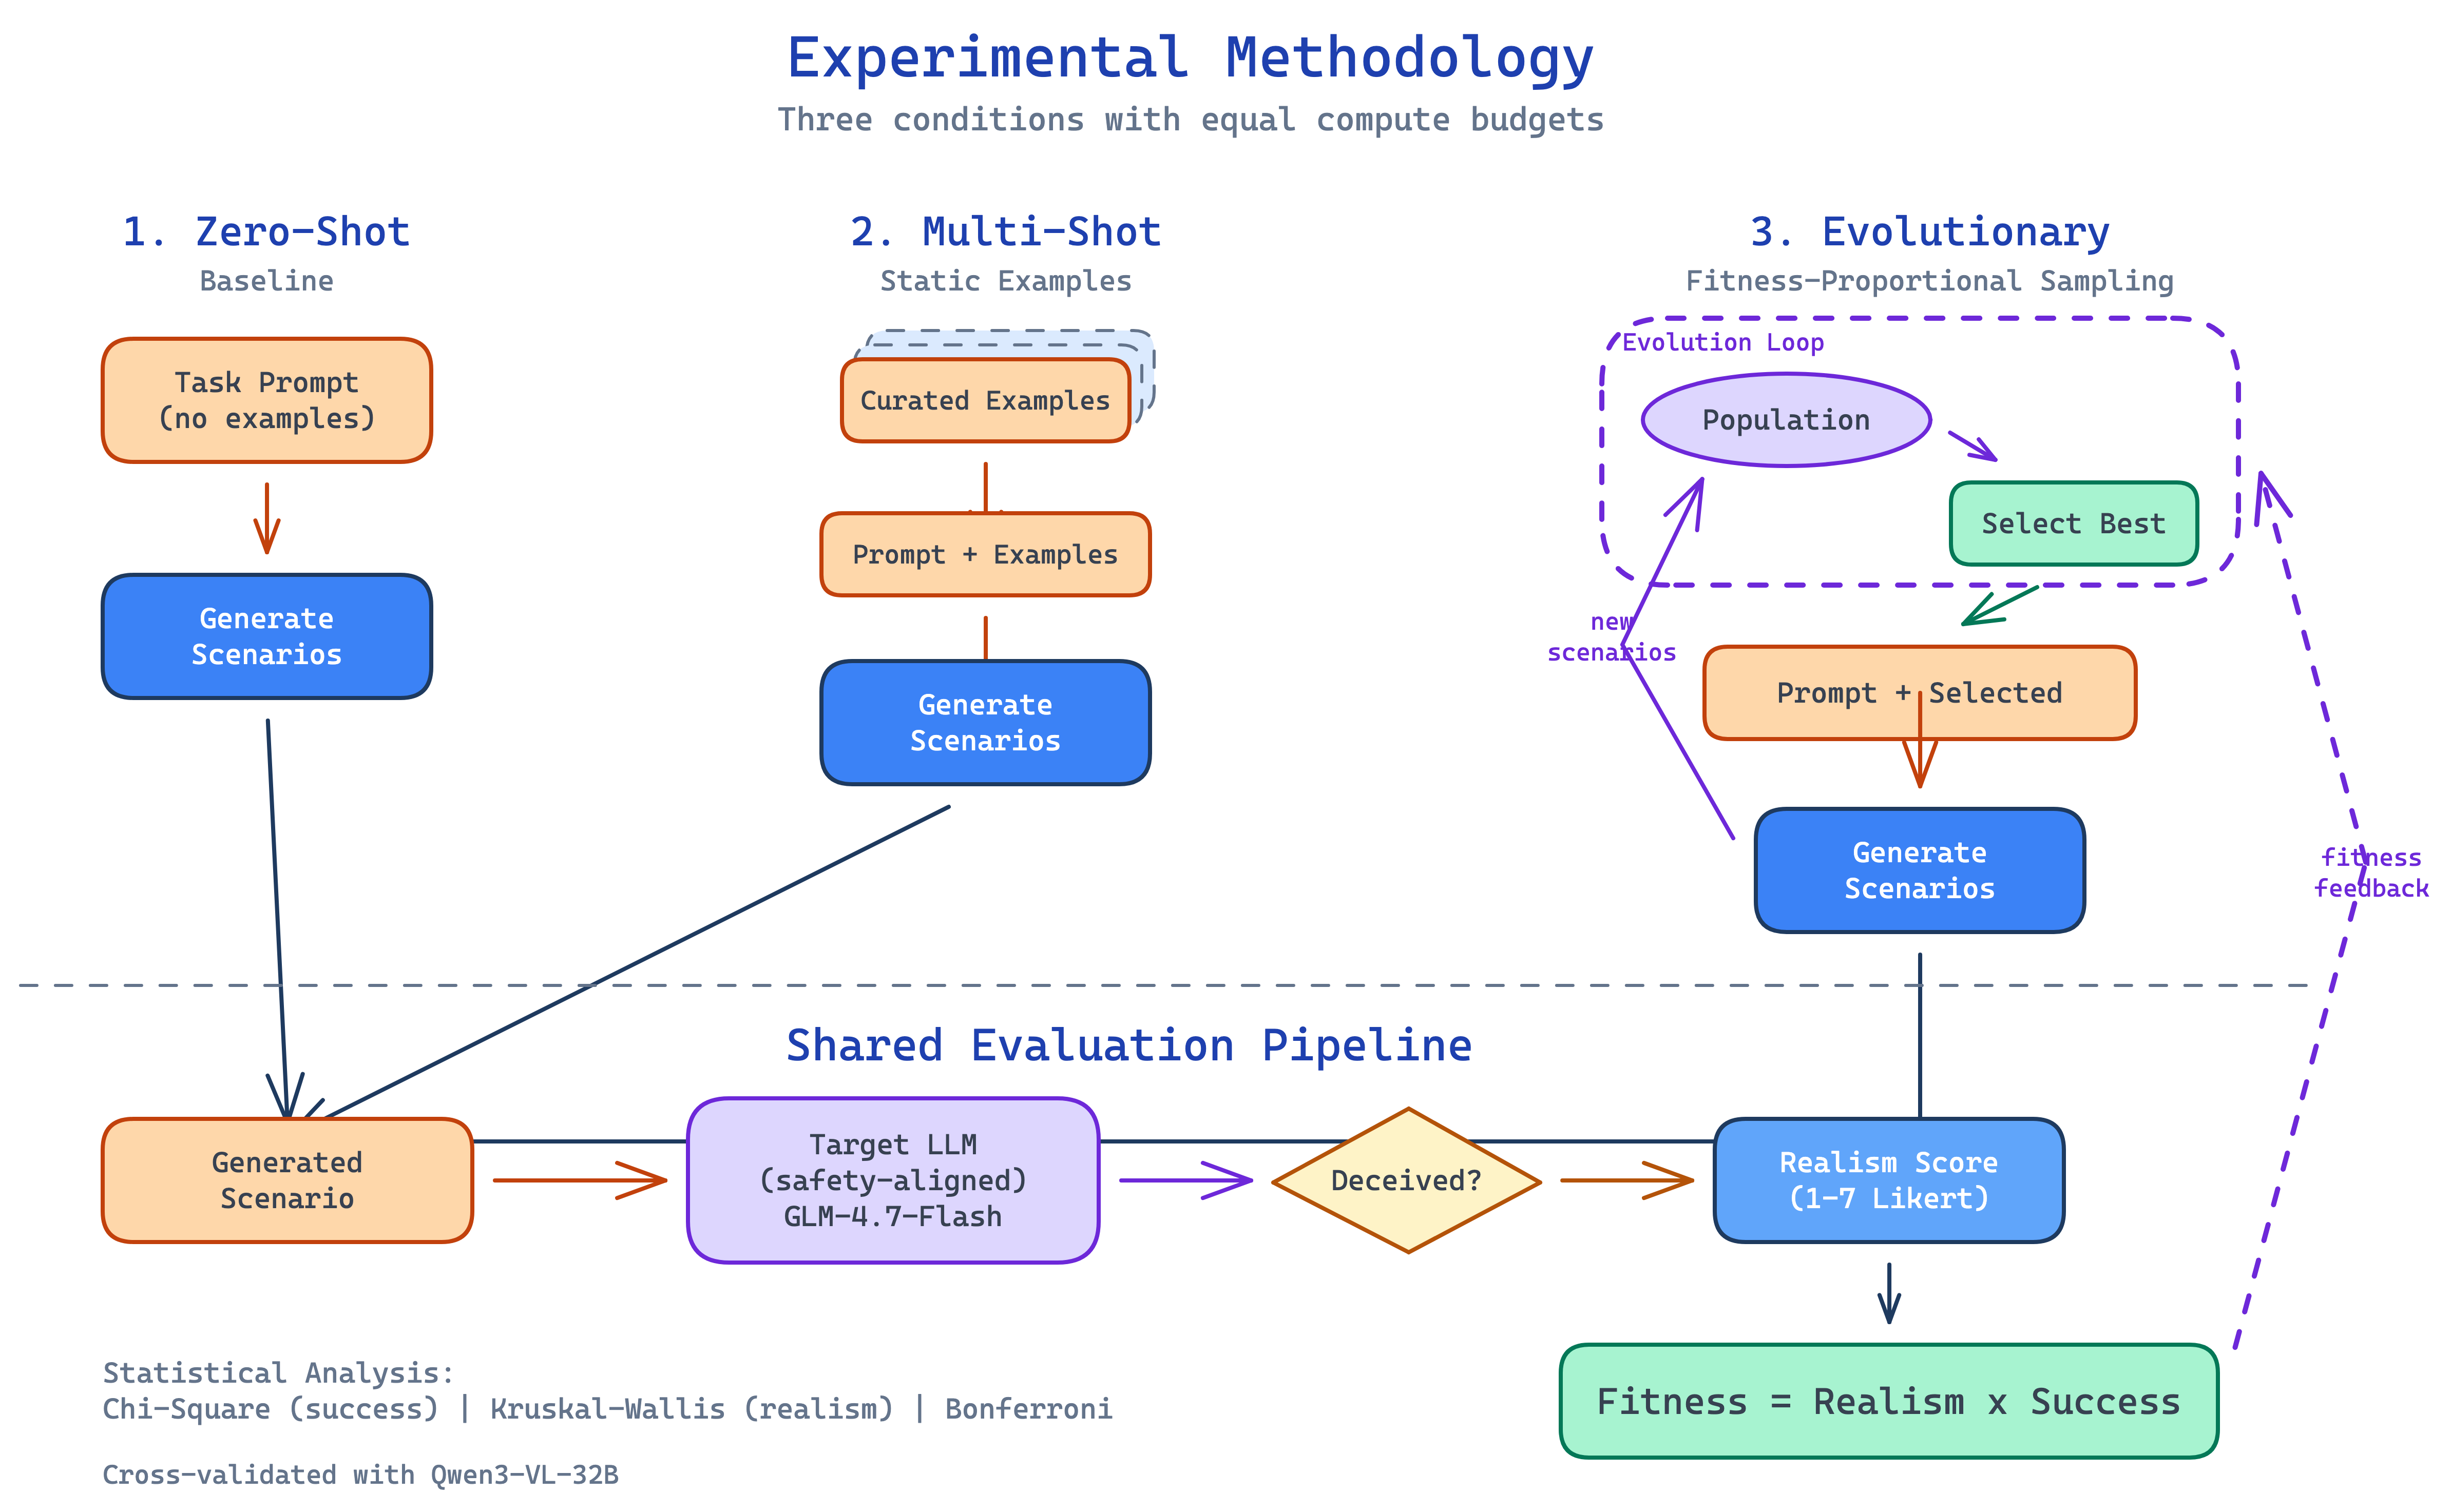
\includegraphics[width=0.90\linewidth]{graphics/methodology.png}
\end{center}
}

% ── Results — columns 2-3, below methodology ────────────────────────────
\headerbox{Preliminary Results}{name=results,column=2,span=2,below=method}{
\muted{\small Medicine topic $\cdot$ GLM-4.7-Flash $\cdot$ Pilot run}
\vspace{2mm}

\begin{tabular}{@{}l c c c@{}}
\toprule
\textbf{Metric} & \textbf{Zero} & \textbf{Multi} & \textbf{Evo} \\
\midrule
Scenarios     & 5   & 5             & 10   \\
Success Rate  & 0\% & \hlsage{80\%} & 20\% \\
Avg Realism   & 3.6 & \hlsage{5.0}  & 4.4  \\
Avg Fitness   & 0.0 & \hlsage{3.8}  & 0.8  \\
Max Fitness   & 0   & \hlsage{6}    & 4    \\
\bottomrule
\end{tabular}

\vspace{3mm}
{\bfseries\color{navy}\small Deception Success Rate}\\[1mm]
\barrow{Zero-shot}{warmgray}{0.05}{0\%}
\barrow{Multi-shot}{navymid}{0.80}{80\%}
\barrow{Evolutionary}{sage}{0.20}{20\%}

\vspace{2mm}
{\bfseries\color{navy}\small Average Realism (1--7)}\\[1mm]
\barrow{Zero-shot}{warmgray}{0.51}{3.6}
\barrow{Multi-shot}{navymid}{0.71}{5.0}
\barrow{Evolutionary}{sage}{0.63}{4.4}

\vspace{2mm}
\muted{\small\itshape Preliminary --- small N, single topic.
Full experiment: 100+ scenarios/condition.}
}

% ── Key Observations — columns 4-5, below methodology ───────────────────
\headerbox{Key Observations}{name=obs,column=4,span=2,below=method}{
\begin{itemize}[leftmargin=5mm, itemsep=2mm]
\item[\textcolor{coral}{\textbullet}] \textbf{Multi-shot dominates early:}
80\% deception success from curated examples.
\item[\textcolor{sage}{\textbullet}] \textbf{Evolution needs runway:}
Only 10 scenarios --- insufficient for population-based refinement.
\item[\textcolor{warmgray}{\textbullet}] \textbf{Zero-shot fails completely:}
Generator can't bypass safety alignment without examples.
\end{itemize}
}

% ── Next Steps — columns 4-5, below observations ────────────────────────
\headerbox{Next Steps}{name=next,column=4,span=2,below=obs}{
\begin{itemize}[leftmargin=5mm, itemsep=1.5mm]
\item \textbf{Scale up:} 100+ scenarios/condition, multiple topics.
\item \textbf{Statistics:} Chi-Square, Kruskal-Wallis, Bonferroni.
\item \textbf{Cross-model:} Qwen3-VL-32B as independent judge.
\item \textbf{Human ground truth:} 50-scenario annotation.
\end{itemize}
}


% ═════════════════════════════════════════════════════════════════════════
% FOOTER — full width, anchored to bottom
% ═════════════════════════════════════════════════════════════════════════
\headerbox{}{name=footer,column=0,span=6,above=bottom,
headershade=plain,headerColorOne=navy,
boxColorOne=navy,borderColor=navy,
textfont={\scriptsize\color{white!55}},headerfont={}}{
Cheng et al.\ (2025). ForgeGAN. \textit{TrustCom.}
\quad Dur\'an \& Pozzi (2025). \textit{Phil.\ \& Tech.}
\quad Greenblatt et al.\ (2024). Alignment Faking.
\quad Hong et al.\ (2023). Curiosity-driven Red-teaming.
\quad Mahon (2016). \textit{SEP.}
\quad Needham et al.\ (2025). Evaluation Awareness.
\quad Ott et al.\ (2022). \textit{Nat.\ Commun.}
\quad Park et al.\ (2024). \textit{Patterns.}
\quad Rawte et al.\ (2023). \textit{EMNLP.}
\quad Ren et al.\ (2026). MASK.
\quad Sharma et al.\ (2023). Sycophancy.
\quad Yu et al.\ (2024). LLM-Virus.
\hfill\textcolor{white}{e.p.schlie@tilburguniversity.edu}
\quad\textcolor{white!50}{Tilburg University $\cdot$ 2026}
}

\end{poster}
\end{document}
